\documentclass[a4paper,14pt]{article}
\usepackage{amsmath}
\usepackage{tikz}
\usepackage{simpler-wick}
\usepackage[UTF8]{ctex}
\usepackage{geometry}
\usepackage[compat=1.1.0]{tikz-feynman}
\usepackage{braket}

\geometry{left=2.0cm,right=2.0cm,top=2.0cm,bottom=2.0cm}

\begin{document}
    \title{格林函数}
    \author{李成蹊}
    \maketitle
    \section{凝胶模型中的电子-电子相互作用}
    讨论金属中电子的元激发特征,能带效应不重要。可以把晶格的正离子近似当做是均匀抹平的连续正电荷分布,类似于凝胶。公共电子则在此正电荷背景上运动,整个系统保持电中性。这种简化的金属电子模型叫做凝胶模型

    电子系统的哈密顿
    \begin{equation*}
        H=\sum_{i=1}^{N}-\frac{\hbar^2}{2m}\nabla_i^2+\frac{1}{2}\sum_{i,j}\frac{e^2}{|r_i-r_j|}+H_+
    \end{equation*}
    $H_+$是均匀分布的正电子背景,包括正电子背景的自能和它与电子的互能。假设共价电子一共有$N$个。记$r=r_i-r_j$对两体势函数做傅里叶变换得到
    \begin{equation*}
        \frac{e^2}{r}=\frac{1}{V}\sum_qV(q)e^{-iq\cdot r}
    \end{equation*}
    \begin{equation*}
        \begin{split}
            V(q)&=\int \mathrm{d}^3r\frac{e^2}{r}e^{iq\cdot r}\\
            &=\int_{0}^{2\pi}\mathrm{d}\varphi\int_{0}^{\pi}\mathrm{d}\theta\int_{0}^{+\infty}r^2\sin\theta\mathrm{d}r\frac{e^2}{r}e^{iq\cdot r}\\
            &=2\pi e^2\int_{0}^{+\infty}\mathrm{d}r\frac{e^{iqr}-e^{-iqr}}{iq}\\
            &=\frac{4\pi e^2}{q^2}
        \end{split}
    \end{equation*}
    所以二次量子化后的哈密顿形式为
    \begin{equation*}
        H=\sum_{k,\sigma}\epsilon_kc_{k,\sigma}^\dagger c_{k,\sigma}+\frac{1}{2}\sum_{q\neq 0}\sum_{k,k',\sigma,\sigma'}V(q)c_{k+q,\sigma}^\dagger c_{k'-q,\sigma'}^\dagger c_{k',\sigma'}c_{k,\sigma}
    \end{equation*}
    凝胶模型要求$q\neq0$,因为$q=0$项与正电背景相互抵消。
    \section{电声相互作用}
    简单晶格只有声频支电子振动,电子与晶格振动的相互作用就是电子与声频声子的相互作用。假设$l$格点上的离子与$j$电子之间的相互作用势能为$V(r_j-l)$. 离子不动时电子与离子相互作用为
    \begin{equation*}
        H^0_{ei}=\sum_{j,l}V(r_j-l)
    \end{equation*}
    这表示电子在周期场中的势能,$l=R_l=\sum_{i}l_ia_i$. 实际上,离子在不断振动,相对位移

\section{S矩阵}
哈密顿可以写成非微扰部分和微扰部分的求和
\begin{equation*}
    H=H_0+V(t)
\end{equation*}
在相互作用表象下
\begin{equation*}
    |\psi(t)\rangle_{I}=e^{iH_0t}|\psi(t)\rangle=e^{iH_0t}e^{-iHt}|\psi(0)\rangle
\end{equation*}
$|\psi(t)\rangle_I$是相互作用绘景下的态函数。带入薛定谔方程得到
\begin{equation*}
    i\frac{\partial}{\partial t}|\psi(t)\rangle_I=V_I(t)|\psi(t)\rangle_I
\end{equation*}
其中$V_I(t)=e^{iH_0t}V(t)e^{-iH_0t}$. 定义相互作用下的时间演化算符$U_I(t)$
\begin{equation*}
    U_I(t)e=e^{iH_0t}e^{-iHt}
\end{equation*}
薛定谔方程可以写成
\begin{equation*}
    i\frac{\partial}{\partial t}U_I(t)=V_I(t)U_I(t)
\end{equation*}
通常的办法是无穷迭代写成积分形式
\begin{equation*}
    U_I(t)=1-i\int_0^{t}\mathrm{d}t_1V(t_1)+(-i)^2\int_0^t\mathrm{d}t_1\int_0^{t_1}\mathrm{d}t_2V_I(t_1)V_I(t_2)+\cdots
\end{equation*}
上述积分与时间顺序有关,为了方便引入编时算符$T$. 编时算符作用在一组与时间有关的算符上满足
\begin{equation*}
    T[O(t_1)O(t_2)O(t_3)]=O(t_3)O(t_1)O(t_2),\quad t_3>t_1>t_2
\end{equation*}
引入$\theta(x)$函数
\begin{equation*}
    \theta(x)=\begin{cases}
        1\quad &x>0\\
        0\quad &x<0\\
        \frac{1}{2}\quad&x=0
    \end{cases}
\end{equation*}
对于两个算符的编时乘积,很容易写成$\theta$函数形式
\begin{equation*}
    T[V_I(t_1)V_I(t_2)]=\theta(t_1-t_2)V_I(t_1)V_I(t_2)+\theta(t_2-t_1)V_I(t_2)V_I(t_1)
\end{equation*}
通过编时算符表示的$U_I(t)$为
\begin{equation*}
    U(t)=1+\sum_{n=1}^{\infty}\frac{(-i)^n}{n!}\int_0^{t}\mathrm{d}t_1\int_0^t\mathrm{d}t_2\cdots\int_0^t\mathrm{d}t_nT[V_I(t_1)\cdots V_I(t_n)]
\end{equation*}
最终可以写成
\begin{equation*}
    U_I(t)=T\left[e^{-i\int_0^t\mathrm{d}t'V_I(t')}\right]
\end{equation*}
我们现在考虑相互作用绘景里从$t'$演化到$t$的过程
\begin{equation*}
    |\psi(t)\rangle_I=S(t,t')|\psi(t')\rangle_I
\end{equation*}
从最初的定义
\begin{equation*}
    |\psi(t)\rangle_I=U_I(t)|\psi(0)\rangle_I=S(t,t')U(t')|\psi(0)\rangle_I
\end{equation*}
所以有
\begin{equation*}
    S(t,t')=U_I(t)U_I^\dagger(t')
\end{equation*}
$S$矩阵满足三个性质
\begin{enumerate}
    \item $S(t,t)=1$
    \item $S^\dagger(t,t')=U_I(t')U_I^\dagger(t)=S(t',t)$
    \item $S(t,t')S(t',t'')=S(t,t'')$
\end{enumerate}
由于
\begin{equation*}
    i\frac{\partial}{\partial t}|\psi(t)\rangle_I=V_I(t)|\psi(t)\rangle_I\Rightarrow i\frac{\partial}{\partial t}S(t,t')|\psi(t')\rangle_I=V_I(t,t')U_I(t,t')|\psi(t')\rangle_I
\end{equation*}
得到$S$矩阵的Dyson解
\begin{equation*}
    S(t,t')=T[e^{-i\int_{t'}^{t}\mathrm{d}t_1V_I(t_1)}]
\end{equation*}
值得注意$t=0$时刻$|\psi(0)\rangle$在三种绘景中对应同一个态。在零温时仅仅只有基态波函数是特别感兴趣的。对于格林函数很有必要定义$|\psi(0)\rangle$为精确的基态波函数$|\Omega\rangle$。因为总哈密顿为$H$,精确的基态$|\Omega\rangle$有总哈密顿的最低能量本征值。但在最开始基态或者基态本征值是不知道的。事实上我们尝试用格林函数来获得精确的信息。

有一个问题,基态波函数$|\Omega\rangle$的形式还不清楚。在相互作用表象里$H_I=H_0+V_I(t)$. $H_0$选择的足够简单,以至于我们能获得它的本征值和本征态。设$H_0$的最小本征值(基态)的本征态为$|0\rangle$. 未知基态波函数$|\Omega\rangle$必须以已知波函数$|0\rangle$的形式确定

在零温时两个基态$|0\rangle$和$|\Omega\rangle$之间的关系由Gell-Mann和Low建立
\begin{equation*}
    |\Omega\rangle=S(0,-\infty)|0\rangle
\end{equation*}
当$t\to+\infty$时
\begin{equation*}
    |\psi(+\infty)\rangle=S(+\infty,0)|\Omega\rangle
\end{equation*}
我们希望从$t=-\infty$绝热演化到$t=+\infty$时波函数与遥远过去态的波函数$|0\rangle$只相差一个相位因子
\begin{equation*}
    |\psi(+\infty)\rangle=e^{i\theta}|0\rangle
\end{equation*}
\begin{equation*}
    e^{i\theta}=\langle0|S(+\infty,-\infty)|0\rangle
\end{equation*}
\section{格林函数}
零温电子格林函数定义为
\begin{equation*}
    G(\lambda,t-t')=-i\langle\Omega|T[c_\lambda(t)c_\lambda^\dagger(t')]|\Omega\rangle
\end{equation*}
量子数$\lambda$是对应问题所感兴趣的量子数。对于自由电子气体我们一般采用$\lambda=(p,\sigma)$. 在零温时,$|\Omega\rangle$一定是基态。如果对应问题的哈密顿选择的是$H$,$|\Omega\rangle$则是$H$的基态,因此它是$H$的本征态。

当然,一开始$H$的基态或者其他本征态是未知的因为这是由格林函数决定的。$H=H_0+V_I(t)$,$H_0$是非微扰部分,$V_I(t)$是相互作用部分。选取的$H_0$一般是基态好求的。现在我们选择一组$H_0$的完全集态,$C_\lambda$表示$H_0$的态,然而$|\Omega\rangle$是$H$的基态。如果我们定义在海森堡表象中,$|\Omega\rangle$与时间无关,但$C_\lambda(t)$通常有
\begin{equation*}
    c_\lambda(t)=e^{iHt}c_\lambda e^{-iHt}
\end{equation*}
为了理解格林函数,我们考虑一个简单情况,对于$t>t'$时
\begin{equation*}
    G(\lambda,t-t')=-i\langle\Omega|c_\lambda(t)c_\lambda^\dagger(t')|\Omega\rangle
\end{equation*}
表示在$t'$时刻产生一个激发$\lambda$,在$t$时刻消灭相同的激发。现在我们假设$\lambda$是$H$的本征值
\begin{equation*}
    Hc_\lambda^\dagger|\Omega\rangle=\epsilon_\lambda c_\lambda^\dagger|\Omega\rangle,\quad H|\Omega\rangle=\epsilon_0|\Omega\rangle,\quad c_\lambda^\dagger|\Omega\rangle=|\lambda\rangle
\end{equation*}
传播子可以写成
\begin{equation*}
    \begin{split}
        G(\lambda,t-t')&=-i\langle\Omega|e^{iHt}c_\lambda e^{-iHt}e^{iHt'}c_\lambda^\dagger e^{-iHt'}|\Omega\rangle\\
        &=-ie^{-i(\epsilon_\lambda-\epsilon_0)(t-t')}
    \end{split}
\end{equation*}
一般来说,$\lambda$不是$H$的本征态,$\lambda$态的粒子会发生散射,经历$t-t'$时间后,有能量平移。

对于另一个时间顺序$t<t'$
\begin{equation*}
    G(\lambda,t-t')=i\langle\Omega|c_\lambda^\dagger(t')c_\lambda(t)|\Omega\rangle
\end{equation*}
由于费米子反对易关系,时间顺序交换费米子算符时会多出一个负号。现在点在在$t$时刻从基态湮灭,在$t'$时刻产生,这对于零温基态是可能的。一种情况是可能的,这种情况对应的基态是金属的费米球。$t$时刻湮灭一个电子,通俗一点讲就是在费米球上移除一个电子,这个湮灭产生一个空穴,空穴可以有相互作用并且在$t-t'$间隔内发生散射。$C_\lambda^\dagger$作用在$t'$时刻上,湮灭这个空穴态$\lambda$.

下一步是把定义在海森堡绘景下的格林函数转化到相互作用绘景中去。我们令$|0\rangle$表示$H_0$的基态
\begin{equation*}
    |\Omega\rangle=S(0,-\infty)|0\rangle
\end{equation*}
带入之前的Gell-Mann Low形式得到格林函数在相互作用绘景中的形式
\begin{equation*}
    G(\lambda,t-t')=-i\frac{\langle0|T[c_\lambda(t)c_\lambda^\dagger(t')S(+\infty,-\infty)]|0\rangle}{\langle0|S(+\infty,-\infty)|0\rangle}
\end{equation*}
这是我们想要的结果,$S(+\infty,-\infty)$放在分子的哪个位置并不重要,因为编时算符将各个部分放在正确的位置。

一个特殊的情况是非微扰格林函数,或者叫做自由格林函数。这种情况下,$V=0$,此时$S=1$
\begin{equation*}
    G^{(0)}(\lambda,t-t')=-i\langle 0|T[c_\lambda(t)c_\lambda^\dagger(t')]|0\rangle
\end{equation*}
对于电子系统有两种不同类型的情况。这两种情况有不同的基态真空$|0\rangle$,并且也有不同的真实真空$|\Omega\rangle$.
\begin{enumerate}
    \item 空带情况。在这里,我们研究了一个电子在其唯一电子所在的能带上的性质。一个例子是半导体或绝缘体导带中的电子。在这种情况下,基态是粒子真空,记作$|0\rangle$。这个基态有性质
    \begin{equation*}
        c_p|0\rangle=0,\quad a_q|0\rangle=0
    \end{equation*}
    其中两个算符分别代表电子和声子的湮灭算符。因此$H_0$和$V$作用在$|0\rangle$得到的是$0$. 这也就是说明$S(t,-\infty)|0\rangle=|0\rangle$

    此时格林函数为
    \begin{equation*}
        G(\lambda,t-t')=-i\theta(t-t')\langle0|c_\lambda(t)c_\lambda^\dagger(t')|0\rangle
    \end{equation*}
    非微扰哈密顿非常容易计算
    \begin{equation*}
        \begin{split}
            G^{(0)}&=-i\theta(t-t')e^{-i\epsilon_\lambda(t-t')}\langle 0|c_\lambda c_\lambda^\dagger|0\rangle\\
            &=-i\theta(t-t')e^{-i\epsilon_\lambda(t-t')}
        \end{split}
    \end{equation*}
    傅里叶变换得到
    \begin{equation*}
        G(\lambda,E)=\int_{-\infty}^{+\infty}\mathrm{d}t e^{iEt}G(\lambda,t)
    \end{equation*}
    为了让积分收敛引入无穷小因子$\eta=0^+$
    \begin{equation*}
        G^{(0)}(\lambda,E)=-i\int_0^{+\infty}\mathrm{d}te^{i(E-\epsilon_\lambda+i\delta)t}
    \end{equation*}
    \begin{equation*}
        G^{(0)}(\lambda,E)=\frac{1}{E-\epsilon_\lambda+i\delta}
    \end{equation*}
    \item 简并电子气体,另一种情况是电子基态在零温时处于费米球状态。最简单的例子就是金属自由电子。系统有化学势$\mu$,所有$E<\mu$的电子态都是占据的。如果非微扰电子($H_0$)的能量用$\epsilon_k$来表示,基态$|0\rangle$表示所有$\epsilon_k<\mu$的态都是满占据的,所有$\epsilon_k>\mu$的态都是空占据的。处理电子相对于化学势的能量,定义$\xi_k=\epsilon_k-\mu$是方便和常规的。对于费米球表面的费米波矢$k_F$
    \begin{equation*}
        \begin{split}
            \langle0|c_k^\dagger c_k|0\rangle&=\theta(k_F-k)\\
            \langle0|c_kc_k^\dagger|0\rangle&=\theta(k-k_F)
        \end{split}
    \end{equation*}
    更一般的表述方式
    \begin{equation*}
        \langle0|c_k^\dagger c_k|0\rangle=\theta(-\xi_k)=\lim_{\beta\to+\infty}\frac{1}{e^{\beta\xi_k+1}}=n_F(\xi_k)
    \end{equation*}
    非微扰格林函数可以写成
    \begin{equation*}
        \begin{split}
            G^{(0)}(\lambda,t-t')&=-i\theta(t-t')\langle0|c_k(t)c_k^\dagger(t')|0\rangle+i\theta(t'-t)\langle0|c_k^\dagger(t')c_k(t)|0\rangle\\
            &=-i\theta(t-t')\langle0|e^{iH_0t}c_ke^{-iH_0(t-t')}c_k^\dagger e^{-iH_0t'}|0\rangle+i\theta(t'-t)\langle0|e^{iH_0t'}c_k^\dagger e^{-iH_0(t'-t)}c_ke^{-iH_0t}|0\rangle\\
            &=-i\theta(t-t')e^{-i\xi_k(t-t')}\theta(\xi_k)+i\theta(t'-t)e^{-i\xi_k(t-t')}\theta(-\xi_k)
        \end{split}
    \end{equation*}
    上式计算利用了
    \begin{equation*}
        e^{iH_0t}c_k e^{-iH_0t}=c_ke^{-iE_kt}
    \end{equation*}
    傅里叶变换为
    \begin{equation*}
        \begin{split}
            G^{(0)}(k,E)&=-i\theta(\xi_k)\int_0^{+\infty}\mathrm{d}te^{i(E-\xi_k+i\eta)t}+i\theta(-\xi_k)\int_{-\infty}^{0}\mathrm{d}te^{i(E-\xi_k-i\eta)}\\
            &=\frac{\theta(\xi_k)}{E-\xi_k+i\eta}+\frac{\theta(-\xi_k)}{E-\xi_k-i\eta}
        \end{split}
    \end{equation*}
    写的紧凑一点为
    \begin{equation*}
        G^{(0)}(k,E)=\frac{1}{E-\xi_k+i\eta\mathrm{sgn}(\xi_k)}
    \end{equation*}
    \item 声子格林函数,声子格林函数定义为
    \begin{equation*}
        D(q,\lambda,t-t')=-i\langle\Omega|T[A_{q\lambda}(t)A_{-q\langle}(t')]|\Omega\rangle
    \end{equation*}
    \begin{equation*}
        A_{q\lambda}=a_{q\lambda}+a_{-q\lambda}^\dagger
    \end{equation*}
    $\lambda$表示声子的极化方向。大多数问题并不需要考虑声子的极化,所以这里我们忽略掉极化指标。
    \begin{equation*}
        D(q,t-t')=-i\frac{\langle0|T[A_{q}(t)A_{-q}(t')]|0\rangle}{\langle0|S(+\infty,-\infty)|0\rangle}
    \end{equation*}
    在零温时,没有声子。基态$|0\rangle$和$|\Omega\rangle$同样是粒子真空$|VAC\rangle$. 非微扰声子格林函数同样的计算方法
    \begin{equation*}
        \begin{split}
            D^{(0)}(q,t-t')&=-i\langle0|T[A_q(t)A_q(t')]|0\rangle\\
            &=-i\langle0|T[(a_qe^{-i\omega_qt}+a_{-q}^\dagger e^{i\omega_qt})(a_{-q}e^{-i\omega_qt'}+a_q^\dagger e^{i\omega_qt'})]|0\rangle
        \end{split}
    \end{equation*}
    零温时
    \begin{equation*}
        \langle0|a_q^\dagger a_q|0\rangle=0,\quad \langle0|a_q a_q^\dagger|0\rangle=1
    \end{equation*}
    零温自由格林函数为
    \begin{equation*}
        D^{(0)}(q,t-t')=-i\theta(t-t')e^{-i\omega_q(t-t')}-i\theta(t'-t)e^{i\omega_q(t-t')}
    \end{equation*}
    傅里叶变换得到
    \begin{equation*}
        \begin{split}
            D^{(0)}(q,\omega)&=\int_{-\infty}^{+\infty}\mathrm{d}t D^{(0)}(q,t)e^{i\omega t}\\
            &=-i\int_{0}^{+\infty}\mathrm{d}te^{i(\omega-\omega_q+i\eta)t}-i\int_{-\infty}^{0}\mathrm{d}te^{i(\omega+\omega_q-i\eta)t}\\
            &=\frac{1}{\omega-\omega_q+i\eta}-\frac{1}{\omega+\omega_q-i\eta}\\
            &=\frac{2\omega_q}{\omega^2-\omega_q^2+i\eta}
        \end{split}
    \end{equation*}
    在非零温情况下声子的热力学平均应该是占据数
    \begin{equation*}
        \begin{split}
            &\langle a_qa_q^\dagger\rangle=N_q+1\\
            &\langle a_q^\dagger a_q\rangle=N_q=\frac{1}{e^{\beta\omega_q}+1}
        \end{split}
    \end{equation*}
    有限温度格林函数
    \begin{equation*}
        \begin{split}
            D^{(0)}(q,t-t')&=-i\theta(t-t')\langle a_q a_q^\dagger\rangle e^{-i\omega_q(t-t')}-i\theta(t'-t)\langle a_q^\dagger a_q\rangle e^{-i\omega_q(t-t')}-i\theta(t-t')\langle a_{-q}^\dagger a_{-q}\rangle e^{i\omega_q(t-t')}\\
            &=-i\theta(t'-t)\langle a_{-q}a_{-q}^\dagger\rangle e^{i\omega_q(t-t')}\\
            &=-i(N_q+1)e^{-i\omega_q|t-t'|}-iN_qe^{i\omega_q|t-t'|}
        \end{split}
    \end{equation*}
\end{enumerate}
\section{Wick定理}
$S$矩阵可以写成
\begin{equation*}
    S(t,t')=Te^{-i\int_{t'}^{t}\mathrm{d}t_1V_I(t_1)}=1+\sum_{n=1}^{+\infty}\frac{(-i)^n}{n!}\int_0^{t}\mathrm{d}t_1\int_0^{t}\mathrm{d}t_1\cdots\int_0^{t}\mathrm{d}t_nT[V_I(t_1)V_I(t_2)\cdots V_I(t_n)]
\end{equation*}
带入Gell-Mann Low表达式中
\begin{equation*}
    G(p,t-t')=\sum_{n=0}^{+\infty}\frac{(-i)^{n+1}}{n!}\int_{-\infty}^{+\infty}\mathrm{d}t_1\cdots\int_{-\infty}^{+\infty}\mathrm{d}t_n\frac{\langle0|T[c_p(t)V_I(t_1)V_I(t_2)\cdots V_I(t_n)c_p(t')]|0\rangle}{\langle0|S(-\infty,+\infty)|0\rangle}
\end{equation*}
分母对应的是极化图,先看分子,例如$\langle0|c_p(t)V_I(t_1)V_I(t_2)V_I(t_3)c_p(t')|0\rangle$

假设$V_I(t_1)$是电子-电子相互作用
\begin{equation*}
    V_I(t_1)=\frac{1}{2}\sum_{k,k,q,\sigma,\sigma'}\frac{4\pi e^2}{q}c_{k+q,\sigma}^\dagger c_{k'-q,\sigma'}^\dagger c_{k',\sigma'}c_{k,\sigma} e^{i(\xi_{k+q}+\xi_{k'-q}-\xi_k-\xi_k')t}
\end{equation*}
在上述的情况里,编时乘积内有7个产生算符和7个湮灭算符。计算这个是非常难办的,特别是高阶计算,涉及到$n$个产生湮灭算符的编时乘积在基态下的平均。
\begin{equation*}
    \langle0|Tc_{1}(t_1)c_{1'}^\dagger(t_1)\cdots c_n(t_n)c_{n'}^\dagger(t_n)|0\rangle
\end{equation*}
我们注意到
\begin{equation*}
    \langle 0|Tc_\alpha(t_1)c_\beta^\dagger(t_2)|0\rangle=\delta_{\alpha,\beta}\langle0|c_\alpha(t_1)c_\alpha^\dagger(t_2)|0\rangle
\end{equation*}
同样的
\begin{equation*}
    \langle0|Tc_\alpha(t_1)c_\beta^\dagger(t_1)c_\gamma(t_2)c_\delta^\dagger(t_2)|0\rangle
\end{equation*}
只有在$\alpha=\beta,\gamma=\delta$或者$\alpha=\delta,\beta=\gamma$的情况下才非$0$. 这样我们希望把复杂编时乘法分解成一个个配对后的编时乘法平均。这样就引入了Wick定理:
\begin{equation*}
    \begin{split}
        \langle 0|Tc_\alpha(t)c_\beta^\dagger(t_1)c_\gamma(t_2)c_\delta^\dagger(t')|0\rangle&=\langle 0|Tc_\alpha(t)c_\beta^\dagger(t_1)|0\rangle\langle0|Tc_\gamma(t_2)c_\delta^\dagger(t')|0\rangle-\langle0|Tc_\alpha(t)c_\delta(t')|0\rangle\langle0|c_\gamma(t_2)c_\beta^\dagger(t_1)|0\rangle\\
        &=\delta_{\alpha,\beta}\delta_{\gamma,\delta}\langle0|c_\alpha(t)c_\alpha^\dagger(t_1)|0\rangle\langle0|c_\gamma(t_2)c_\gamma^\dagger(t')|0\rangle-\delta_{\alpha,\delta}\delta_{\beta,\gamma}\langle0|c_\alpha(t)c_\delta^\dagger(t')|0\rangle\langle0|c_\gamma(t_2)c_\beta(t_1)|0\rangle
    \end{split}
\end{equation*}
Wick定理指出,在产生湮灭算符之间的所有可能配对中,每对算符符都应该是按时序排列的。每一对的时序给出了整个结果的固有时间顺序。

有三条规则值得注意:
\begin{enumerate}
    \item Wick收缩的时候费米子算符交换位置需要增加一次负号,奇数次交换结果为负,偶数次交换结果不变,例如上例的负号。
    \item 第二条规则涉及代表不同激发算子的组合的时间顺序。例如电声相互作用中
    \begin{equation*}
        \langle0|Tc_p(t)c_{p_1}(t_1)A_{q_1}(t_1)c_{p_2}(t_2)c_{p_3}^\dagger(t_3)A_{q_2}(t_2)|0\rangle
    \end{equation*}
    由于电子算符和声子算符相互对易,所以电子声子之间的顺序无关紧要。这个括号可以理解分解成两个独立的部分,一部分代表电子,一部分代表声子
    \begin{equation*}
        \langle0|Tc_p(t)c_{p_1}(t_1)c_{p_2}(t_2)c_{p_3}^\dagger(t_3)|0\rangle\langle0|A_{q_1}(t_1)A_{q_2}(t_2)|0\rangle
    \end{equation*}
    声子是玻色子,满足对易关系,所以Wick收缩时无需考虑符号问题。
    \item 第三个规则是两个等时算符的编时乘积怎么算,例如
    \begin{equation*}
        \langle0|Tc_{k_1}^\dagger(t_1)c_{k_2}(t_1)|0\rangle
    \end{equation*}
    这种情况下,湮灭算符总是在右边,写成正规乘积
    \begin{equation*}
        \langle0|Tc_{k_1}^\dagger(t_1)c_{k_2}(t_1)|0\rangle=\delta_{k_1,k_2}\langle0|c_{k_1}^\dagger(t_1)c_{k_1}(t_1)|0\rangle=\delta_{k_1,k_2}n_F(\xi_{k_1})
    \end{equation*}
    计算结果是粒子数算符,与时间无关。这个约定依赖于用来表示哈密顿函数的约定。在构建哈密顿时,所有的产生湮灭算符都应该是正规序。

    当两个电子算符不等时配对时,约定把产生算符写在右边
    \begin{equation*}
        \langle0|Tc_{k_1}^\dagger(t_1)c_{k_2}(t_2)|0\rangle=-\delta_{k_1,k_2}\langle0|Tc_{k_1}(t_2)c_{k_1}^\dagger(t)|0\rangle
    \end{equation*}
    立马可以看出这正是非微扰自由格林函数$G^{(0)}(k_1,t_2-t_1)$. Wick收缩得到的所有的项,要么是等时收缩粒子数算符要么是自由格林函数。总之,Wick定理陈述了这样的一个事实,时序乘积括号可以通过展开成各种配对乘积来计算。每一项配对都和自由格林函数或者粒子数算符$n_F,n_B$联系起来。这些展开给出来总的时序乘积的结果。当哈密顿$H_0$这部分是产生湮灭算符的双线性型时,Wick定理总是有效的。这个定理在$H_0$包含成对相互作用时失效。
\end{enumerate}
举个比较简单的例子,$n=2$时的电声相互作用
\begin{equation*}
    \begin{split}
        G(p,t-t')&=G^{(0)}(p,t-t')+(-i)^2\int_{-\infty}^{+\infty}\mathrm{d}t_1\langle0|Tc_{p,\sigma}(t)V(t_1)c_{p,\sigma}^\dagger(t')|0\rangle\\
        &+(-i)^3\int_{-\infty}^{+\infty}\mathrm{d}t_1\int_{-\infty}^{+\infty}\mathrm{d}t_2\langle0|Tc_{p,\sigma}(t)V(t_1)V(t_2)c_{p,\sigma}^\dagger(t')|0\rangle
    \end{split}
\end{equation*}
相互作用为
\begin{equation*}
    V=\sum_{q,k,s}M_qA_qc_{k+q,s}^\dagger c_{k,s}
\end{equation*}
一次项$n=1$对应的结果是$0$,因为
\begin{equation*}
    \langle0|TA_q|0\rangle=0
\end{equation*}
同样的,$n$为奇数时的项都是$0$,只有$n$为偶数项的结果对电声相互作用有贡献
\begin{equation*}
    \begin{split}
        G(p,t-t')&=G^{(0)}(p,t-t')+\frac{(-i)^3}{2!}\int_{-\infty}^{+\infty}\mathrm{d}t_1\int_{-\infty}^{+\infty}\mathrm{d}t_2\sum_{q_1,q_2}M_{q_1}M_{q_2}\langle0|TA_{q_1}(t_1)A_{q_2}(t_2)|0\rangle\\
        &\times\sum_{k_1,k_2,s,s'}\langle0|Tc_{p,\sigma}(t)c_{k_1+q_1,s}^\dagger(t_1)c_{k_1,s}(t_1)c_{k_2+q_2,s'}^\dagger(t_2)c_{k_2,s'}(t_2)c_{p,\sigma}^\dagger(t')|0\rangle
    \end{split}
\end{equation*}
声子收缩给出了自由单声子格林函数
\begin{equation*}
    \langle0|TA_{q_1}(t_1)A_q(t_2)|0\rangle=i\delta_{q_1,-q_2}D^{(0)}(q_1,t_1-t_2)
\end{equation*}
这里注意$A_{-q}=A_q^\dagger$. 电子收缩有六种情况,分别写成六项,值得注意$q_1=-q_2$
\begin{equation*}
    \begin{array}{l}
        \langle0 |T c_{\mathbf{p} \sigma}(t) c_{\mathbf{k}_{1}+\mathbf{q}_{1}, s}^{\dagger} (t_{1} ) c_{\mathbf{k}_{1}, s} (t_{1} ) c_{\mathbf{k}_{2}+\mathbf{q}_{2}, s^{\prime}}^{\dagger} (t_{2} ) c_{\mathbf{k}_{2} s^{\prime}} (t_{2} ) c_{\mathbf{p} \sigma}^{\dagger} (t^{\prime} ) |0\rangle \\
        =\langle0 |T c_{\mathbf{p} \sigma}(t) c_{\mathbf{k}_{1}+\mathbf{q}_{1}, s}^{\dagger} (t_{1} ) |0\rangle \langle0 |T c_{\mathbf{k}_{1}, s} (t_{1} ) c_{\mathbf{k}_{2}+\mathbf{q}_{2}, s^{\prime}}^{\dagger} (t_{2} ) |0\rangle\langle0 |T c_{\mathbf{k}_{2} s^{\prime}} (t_{2} ) c_{\mathbf{p} \sigma}^{\dagger} (t^{\prime} ) |0\rangle \\
        +\langle0 |T c_{\mathbf{p} \sigma}(t) c_{\mathbf{k}_{2}+\mathbf{q}_{2}, s^{\prime}}^{\dagger} (t_{2} ) |0\rangle \langle0 |T c_{\mathbf{k}_{1}, s} (t_{1} ) c_{\mathbf{p}, \sigma}^{\dagger} (t^{\prime} ) |0\rangle\langle0 |T c_{\mathbf{k}_{2}, s^{\prime}} (t_{2} ) c_{\mathbf{k}_{1}+\mathbf{q}_{1}, s}^{\dagger} (t_{1} ) |0\rangle \\
        +\langle0 |T c_{\mathbf{p} \sigma}(t) c_{\mathbf{k}_{1}+\mathbf{q}, s}^{\dagger} (t_{1} ) |0\rangle \langle0 |T c_{\mathbf{k}_{1}, s} (t_{1} ) c_{\mathbf{p} \sigma}^{\dagger} (t^{\prime} ) |0\rangle \langle0 |T c_{\mathbf{k}_{2}+\mathbf{q}_{2}, s^{\prime}}^{\dagger} (t_{2} ) c_{\mathbf{k}_{2} s^{\prime}} (t_{2} ) |0\rangle \\
        +\langle0 |T c_{\mathbf{p} \sigma}(t) c_{\mathbf{k}_{2}+\mathbf{q}_{2}, s^{\prime}}^{\dagger} (t_{2} ) |0\rangle \langle0 |T c_{\mathbf{k}_{2}, s^{\prime}} (t_{2} ) c_{\mathbf{p} \sigma}^{\dagger} (t^{\prime} ) |0\rangle\langle0 |T c_{\mathbf{k}_{1}+\mathbf{q}_{1}, s}^{\dagger} (t_{1} ) c_{\mathbf{k}_{1}, s} (t_{1} ) |0\rangle \\
        +\langle0 |T c_{\mathbf{p} \sigma}(t) c_{\mathbf{p} \sigma}^{\dagger} (t^{\prime} ) |0\rangle \langle0 |T c_{\mathbf{k}_{1}+\mathbf{q}_{1}, s}^{\dagger} (t_{1} ) c_{\mathbf{k}_{1}, s} (t_{1} ) |0\rangle\langle0 |T c_{\mathbf{k}_{2}+\mathbf{q}_{2}, s^{\prime}}^{\dagger} (t_{2} ) c_{\mathbf{k}_{2}, s^{\prime}} (t_{2} ) |0\rangle \\
        -\langle0 |T c_{\mathbf{p} \sigma}(t) c_{\mathbf{p} \sigma}^{\dagger} (t^{\prime} ) |0\rangle \langle0 |T c_{\mathbf{k}_{1}, s} (t_{1} ) c_{\mathbf{k}_{2}+\mathbf{q}_{2}, s^{\prime}}^{\dagger} (t_{2} ) |0\rangle\langle0 |T c_{\mathbf{k}_{2}^{\prime}} (t_{2} ) c_{\mathbf{k}_{1}+\mathbf{q}_{1}, s}^{\dagger} (t_{1} ) |0\rangle
        \end{array}
\end{equation*}
每一个配对括号要么是自由格林函数$G^{(0)}$要么是粒子数算符$n_F$. 进一步计算得到
\begin{equation*}
  \begin{array}{l}
i^{3} \delta_{\mathbf{p}=\mathbf{k}_{2}=\mathbf{k}_{1}+\mathbf{q}_{1}} \delta_{s=s^{\prime}=\sigma} G^{(0)}\left(\mathbf{p}, t-t_{1}\right) G^{(0)}\left(\mathbf{p}-\mathbf{q}_{1}, t_{1}-t_{2}\right) G^{(0)}\left(\mathbf{p}, t_{2}-t^{\prime}\right) \\
\quad+i^{2} \delta_{\mathbf{p}=\mathbf{k}_{1}=\mathbf{k}_{2}-\mathbf{q}_{1}} \delta_{s=s^{\prime}=\sigma} G^{(0)}\left(\mathbf{p}, t-t_{2}\right) G^{(0)}\left(\mathbf{p},+\mathbf{q}_{1}, t_{2}-t_{1}\right) G^{(0)}\left(\mathbf{p}, t_{1}-t^{\prime}\right) \\
\quad+i^{2} \delta_{\mathbf{q}_{1}=0} \delta_{\mathbf{p}=\mathbf{k}_{1}} \delta_{s=\sigma} n_{F}\left(\xi_{\mathbf{k}_{2}}\right) G^{(0)}\left(\mathbf{p}, t-t_{1}\right) G^{(0)}\left(\mathbf{p}, t_{1}-t^{\prime}\right) \\
\quad+i^{2} \delta_{\mathbf{q}_{1}=0} \delta_{\mathbf{p}=\mathbf{k}_{2}} \delta_{s^{\prime}=\sigma} n_{F}\left(\xi_{\mathbf{k}_{1}}\right) G^{(0)}\left(\mathbf{p}, t-t_{2}\right) G^{(0)}\left(\mathbf{p}, t_{2}-t^{\prime}\right) \\
\quad+i \delta_{\mathbf{q}_{1}=0} \delta_{\mathbf{q}_{2}=0} n_{F}\left(\xi_{\mathbf{k}_{1}}\right) n_{F}\left(\xi_{\mathbf{k}_{2}}\right) G^{(0)}\left(\mathbf{p}, t-t^{\prime}\right) \\
-i^{3} \delta_{\mathbf{k}_{1}=\mathbf{k}_{2}-\mathbf{q}_{1}} \delta_{s^{\prime}=s} G^{(0)}\left(\mathbf{p}, t-t^{\prime}\right) G^{(0)}\left(\mathbf{k}_{1}, t_{1}-t_{2}\right) G^{(0)}\left(\mathbf{k}_{1}+\mathbf{q}_{1}, t_{2}-t_{1}\right)
\end{array}
\end{equation*}
\section{费曼图}
电子自由格林函数$G^{(0)(p,t-t')}$用从$t'$到$t$的实线表示,如图所示。箭头一般表示了方向。箭头仅仅是为了方便,并不意味着或者要求$t>t'$. 声子格林函数用虚线表示。由于声子满足
\begin{equation*}
    D^{(0)}(q,t-t')=D^{(0)}(-q,t'-t)
\end{equation*}
所以声子没有标记箭头,声子传播方向与$q$无关。声子在时间上可以被看作是两个方向上的声子。

进一步考虑$\langle0|c_{p,s}^\dagger(t)c_{p,s}(t)|0\rangle$的图
\begin{equation*}
    \langle0|c_{p,s}^\dagger(t)c_{p,s}(t)|0\rangle=n_F(xi_p)
\end{equation*}
占据数$n_F$被绘制为一条实线,它循环形成闭合圆,并表示在同一时间点开始和结束。
\begin{equation*}
    \begin{split}
        G^{(0)}(p,t-t')&=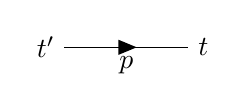
\begin{tikzpicture}
            \begin{feynman}
                \vertex (a) {\(t'\)};
                \vertex [right=2cm of a] (b) {\(t\)};
                \diagram*{(a) -- [fermion,edge label'=\(p\)] (b)};
            \end{feynman}
        \end{tikzpicture}\quad
        D^{(0)}(q,t-t')=\begin{tikzpicture}
            \begin{feynman}
                \vertex (a) {\(t'\)};
                \vertex [right=2cm of a] (b) {\(t\)};
                \diagram*{(a) -- [scalar,edge label'=\(q\)] (b)};
            \end{feynman}
        \end{tikzpicture}\\
        n_F(\xi_p)=\braket{c_p^\dagger(t)|c_p(t)}&=\begin{tikzpicture}
            \begin{feynman}
                \vertex (a);
                \vertex [right=1cm of a] (b);
                \diagram[horizontal=a to b, layered layout, small, baseline=\plusheight]{(a) -- [fermion,half left] (b)};
                \diagram[horizontal=a to b, layered layout, small, baseline=\plusheight]{(b) -- [fermion,half left,edge label'=\(p\)] (a)};
            \end{feynman}
        \end{tikzpicture}\quad\quad\quad\quad\quad\quad\quad\quad\quad
        V(q)=\begin{tikzpicture}
            \begin{feynman}
                \vertex (a);
                \vertex [below=1cm of a] (b);
                \diagram{(a) -- [boson,edge label'=\(q\)] (b)};
            \end{feynman}
        \end{tikzpicture}
    \end{split}
\end{equation*}
通过这些规则,可以把之前求的格林函数展开得到六项画成费曼图,如图所示。费曼图$(a)$到$(f)$依次是上面电声格林函数,每一项都有连接$t_1$到$t_2$的声子线
\begin{equation*}
    \begin{split}
        &(a)\quad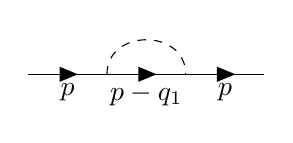
\begin{tikzpicture}
            \begin{feynman}
                \vertex (a);
                \vertex[right=1cm of a] (b);
                \vertex[right=1cm of b] (c);
                \vertex[right=1cm of c] (d);
                \diagram*{(a) --[edge label'=\(p\),fermion] (b)};
                \diagram*{(b) --[edge label'=\(p-q_1\),fermion] (c)};
                \diagram*{(c) --[edge label'=\(p\),fermion] (d)};
                \diagram*{(b) --[scalar,half left] (c)};
            \end{feynman}
        \end{tikzpicture}\quad(b)\quad
    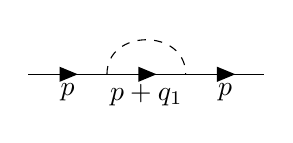
\begin{tikzpicture}
        \begin{feynman}
            \vertex (a);
            \vertex[right=1cm of a] (b);
            \vertex[right=1cm of b] (c);
            \vertex[right=1cm of c] (d);
            \diagram*{(a) --[edge label'=\(p\),fermion] (b)};
            \diagram*{(b) --[edge label'=\(p+q_1\),fermion] (c)};
            \diagram*{(c) --[edge label'=\(p\),fermion] (d)};
            \diagram*{(b) --[scalar,half left] (c)};
        \end{feynman}
    \end{tikzpicture}\\
    &(c)\quad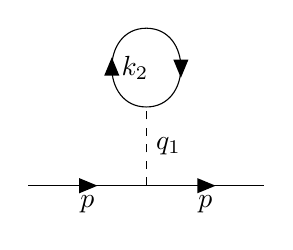
\begin{tikzpicture}
        \begin{feynman}
            \vertex (a);
            \vertex[right=1.5cm of a] (b);
            \vertex[right=1.5cm of b] (c);
            \vertex[above=1cm of b] (d);
            \vertex[above=1cm of d] (e);
            \diagram*{(a) --[fermion,edge label'=\(p\)] (b)};
            \diagram*{(b) --[fermion,edge label'=\(p\)] (c)};
            \diagram*{(b) --[scalar,edge label'=\(q_1\)] (d)};
            \diagram*{(d) --[fermion,edge label'=\(k_2\),half left] (e)};
            \diagram*{(e) --[fermion,half left] (d)};
        \end{feynman}
    \end{tikzpicture}\quad(d)\quad
    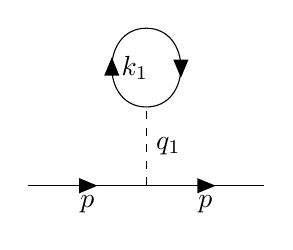
\begin{tikzpicture}
        \begin{feynman}
            \vertex (a);
            \vertex[right=1.5cm of a] (b);
            \vertex[right=1.5cm of b] (c);
            \vertex[above=1cm of b] (d);
            \vertex[above=1cm of d] (e);
            \diagram*{(a) --[fermion,edge label'=\(p\)] (b)};
            \diagram*{(b) --[fermion,edge label'=\(p\)] (c)};
            \diagram*{(b) --[scalar,edge label'=\(q_1\)] (d)};
            \diagram*{(d) --[fermion,edge label'=\(k_1\),half left] (e)};
            \diagram*{(e) --[fermion,half left] (d)};
        \end{feynman}
    \end{tikzpicture}\\
    &(e)\quad
    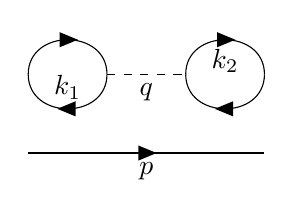
\begin{tikzpicture}
        \begin{feynman}
            \vertex (a);
            \vertex[right=3cm of a] (b);
            \vertex[right=1cm of a] (c);
            \vertex[above=1cm of c] (c1);
            \vertex[above=1cm of a] (d);
            \vertex[left=1cm of b] (e);
            \vertex[above=1cm of e] (e1);
            \vertex[above=1cm of b] (f);
            \diagram*{(a) --[fermion,edge label'=\(p\)] (b)};
            \diagram*{(c1) --[scalar,edge label'=\(q\)] (e1)};
            \diagram*{(c1) --[fermion,half left,edge label'=\(k_1\)] (d)};
            \diagram*{(d) --[fermion,half left] (c1)};
            \diagram*{(e1) --[fermion,half left,edge label'=\(k_2\)] (f)};
            \diagram*{(f) --[fermion,half left] (e1)};
        \end{feynman}
    \end{tikzpicture}\quad(f)\quad
    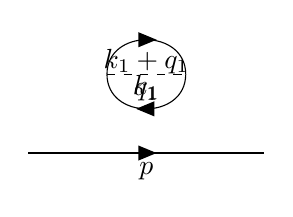
\begin{tikzpicture}
        \begin{feynman}
            \vertex (a);
            \vertex[right=3cm of a] (b);
            \vertex[right=1cm of a] (c);
            \vertex[above=1cm of c] (c1);
            \vertex[left=1cm of b] (d);
            \vertex[above=1cm of d] (d1);
            \diagram*{(a) --[fermion,edge label'=\(p\)] (b)};
            \diagram*{(c1) --[fermion,edge label'=\(k_1+q_1\),half left] (d1)};
            \diagram*{(d1) --[fermion,edge label'=\(k_1\),half left] (c1)};
            \diagram*{(c1) --[scalar,edge label'=\(q_1\)] (d1)};
        \end{feynman}
    \end{tikzpicture}
    \end{split}
\end{equation*}
$(c)$和$(d)$是$0$,因为当声子波矢$q=0$时这一项为$0$. $q=0$的声子要么是晶体的平移,要么永久形变,这两者都不属于哈密顿量。对$q$求和的项应该排除$q=0$项。










\end{document} 